\chapter{Udviklingsforløb} \label{udvikling}
I projektet er det valgt, at benytte en iterativ udviklingsproces. Iterative udviklingsprocesser er særdeles velegnede til projekter, hvor kendskabet til domænet er forholdsvis begrænset. Det har været tilfældet ved denne opgave. Selvom vi begge har deltaget i kurset "Effektelektronik", vurderes det, at den iterative proces ville være god, da kurset var meget analytisk og med overordnet gennemgange af forskellige convertere. Her har vi skullet fordybe os i en specifik converter typologi og desuden realisere den.


Figur~\ref{fig:ASE} viser ASE modellen som projektet har taget udgangspunkt i. 
\begin{figure}[H]
	\center
	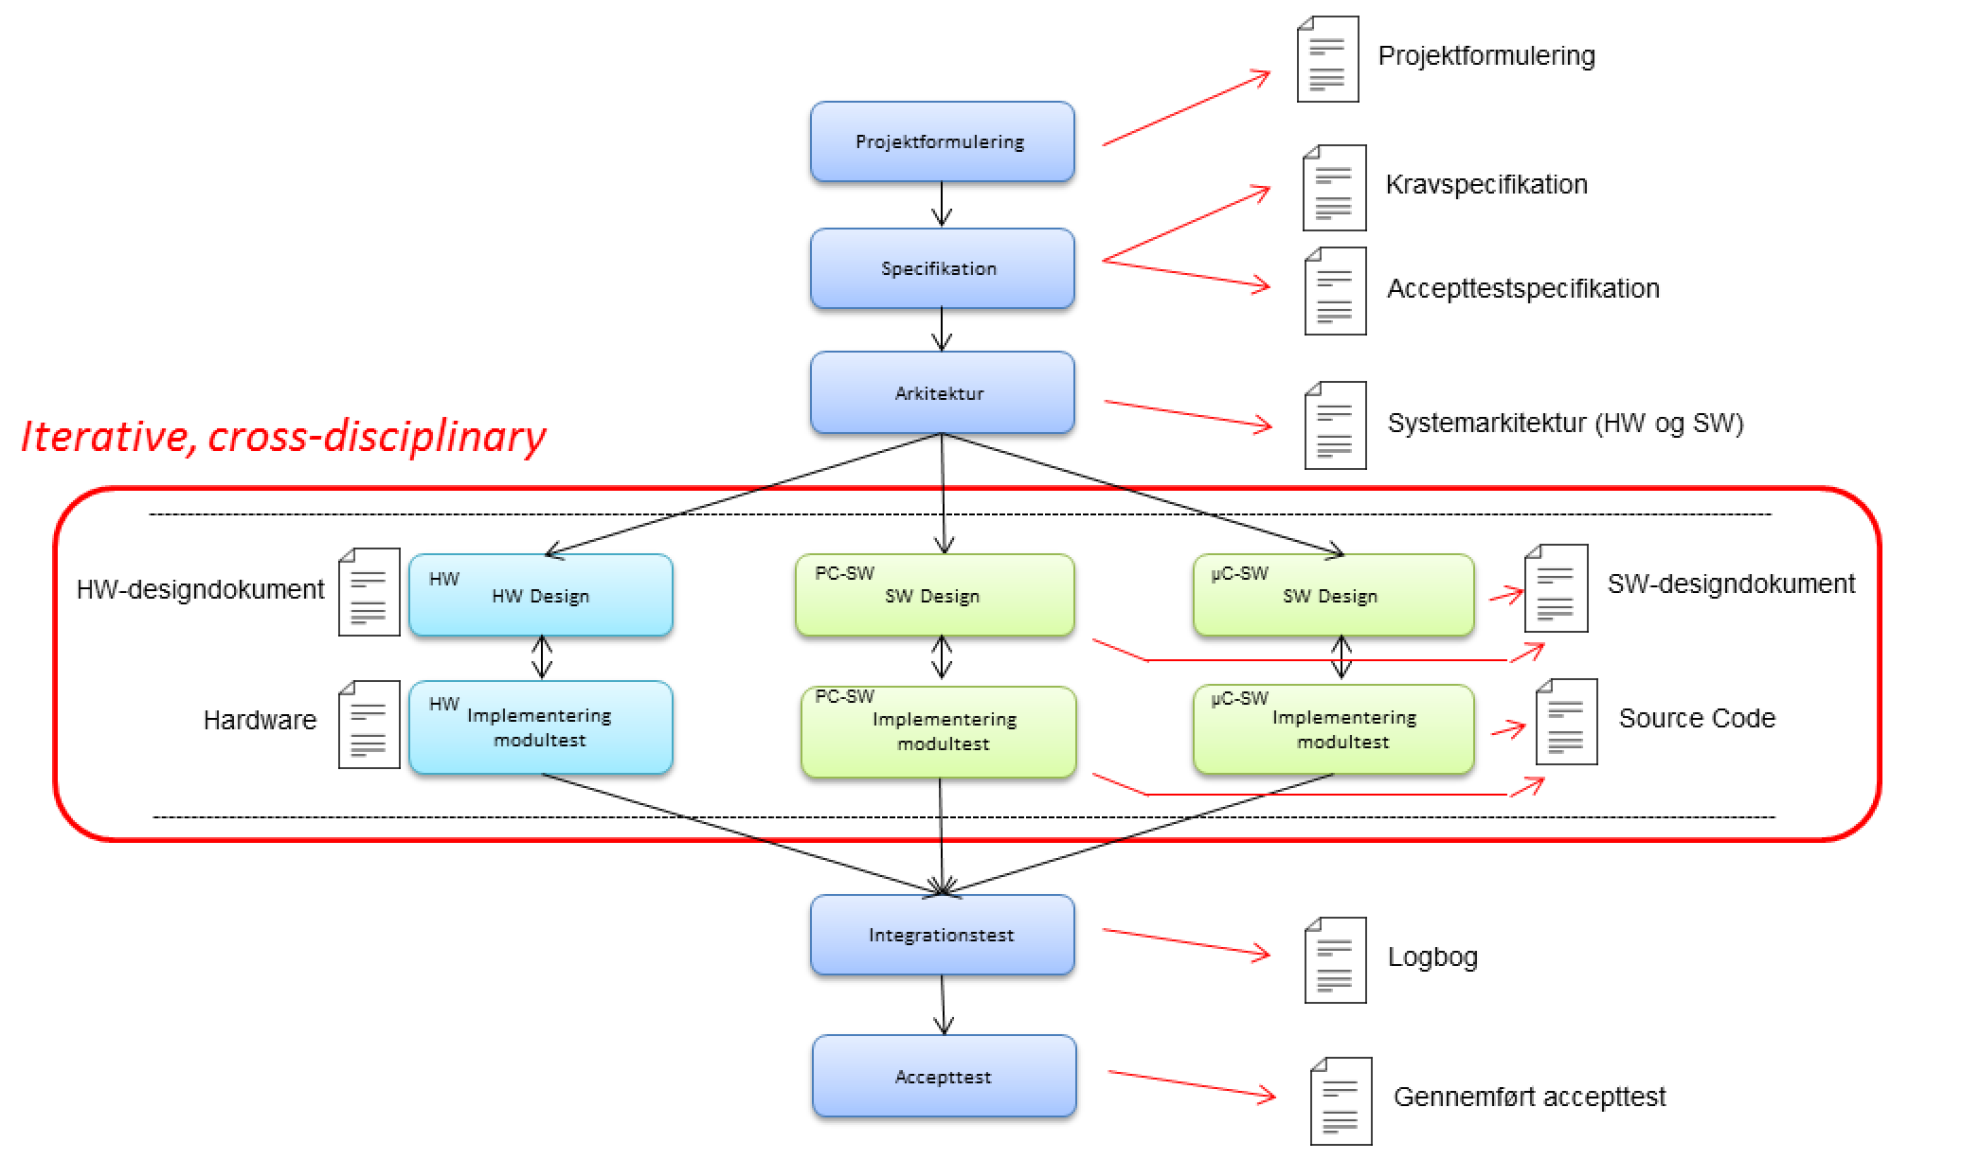
\includegraphics[max width=0.7\linewidth]{/tex/Billeder/ASEmodel.png}
	\caption{ASE model med fokus på iterativ proces~\cite{udviklingsproces}}
	\label{fig:ASE}
\end{figure} 
I begyndelsen blever produktet specificeret med krav, hvilket ikke har været iterativt, som det efterfølgende. Det skyldes at projektet er et oplæg fra Terma, som selv har specificeret kravene, og derfor har de været forholdsvis faste. Der har til dels stadig været krav, som senere i perioden er blevet lavet om efter samtaler mellem Terma og gruppen, men det er begrænset.

Til gengæld er det især design-, implementerings- og modultestfasen, der har fungeret iterativt. Det vil sige, at der forbedres på produktet i små bidder, eftersom der erfares mere og mere fra gang til gang. Ved hver iteration opstilles delmål forinden, som der opfyldes inden næste iteration påbegyndes. 
Til slut er der udarbejdet en accepttest, som kun er blevet udført én gang.

Det vil sige, at selvom der arbejdes iterativt, kan gennemførelsen stadig deles op i flere faser som vist i figur~\ref{fig:Iterative} 
\begin{figure}[H]
	\center
	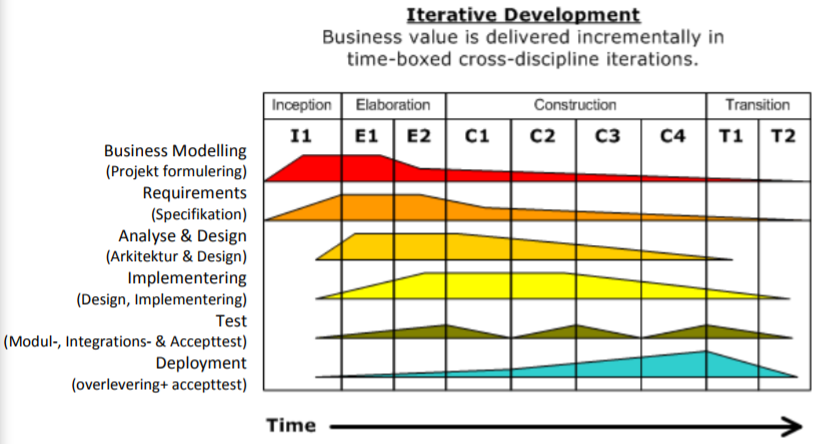
\includegraphics[max width=0.7\linewidth]{/tex/Billeder/Iterative.png}
	\caption{Udviklingsfaser og iterationer~\cite{udviklingsproces}}
	\label{fig:Iterative}
\end{figure} 
Her ses det hvordan design-, implementering- og testfaerne ligger oveni hinanden, mens specificeringen og afsluttende accepttest osv. er i højsædet i hhv. begyndelsen og slutningen.


Til at implementere udviklingsmodellen er det nødvendigt med et projektstyringsværktøj. Her faldt valget på scrum~\cite{Scrum}, da der er god erfaring med dette fra tidligere semesterprojekter. Scrum er henvendt til projektstyring og kan bruges i agile udviklingsprocesser. En del af Scrum går ud på at dele gruppens medlemmer op i mindre grupper med grupperoller. Denne del har ikke givet mening her, med en gruppe på 2. 
Til gengæld optimerer Scrum processen ved at reflektere over processen løbende og produktet deles op i mange små opgaver (backlog items). Opdeling og uddelegering af disse backlog items er for dette projekt gjort på et task board. Et øjebliksbillede af taskboardet kan ses på figur~\ref{fig:Taskboard} 
\begin{figure}[H]
	\center
	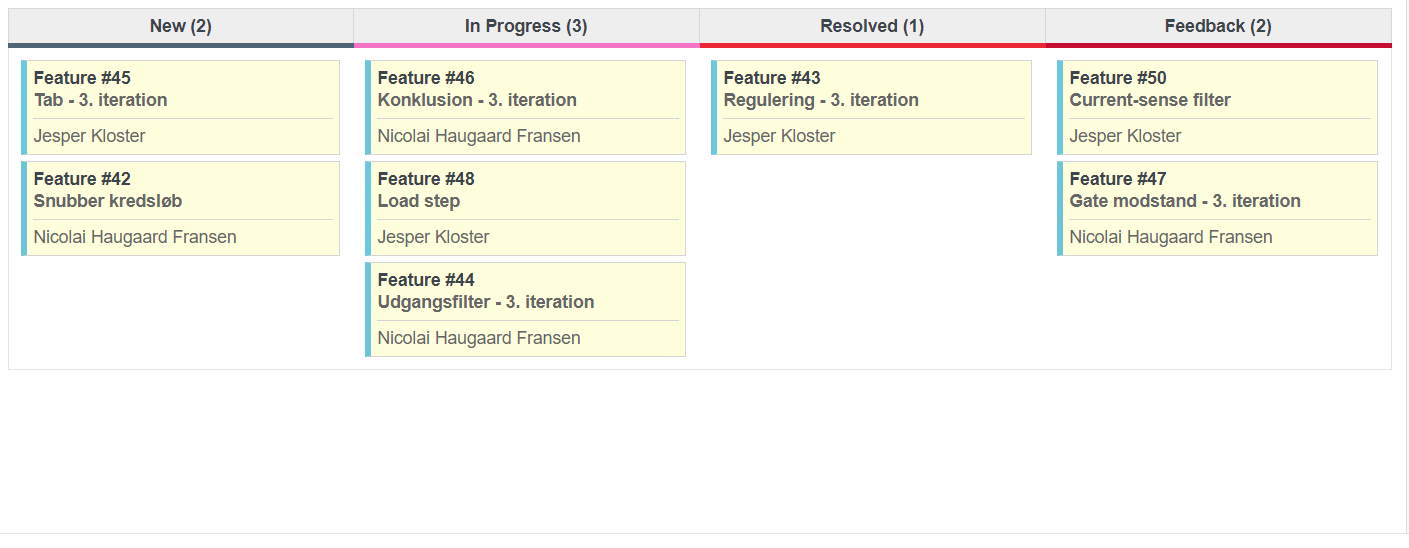
\includegraphics[max width=1\linewidth]{/tex/Billeder/Scrumtask.png}
	\caption{Scrum taskboard}
	\label{fig:Taskboard}
\end{figure} 
Overordnet set er taskboardsne yderligere delt ind i iterationerne. Her kigges på design-, implementering- og designfasens 3. iteration og dets backlog items, som på boardet kaldes features. Et samlet overblik over samtlige iterationer, der er lavet i projektet, er opstillet herunder:

\begin{itemize}
\item Specificering
\item Kravspecifikation
\item Systemarkitektur
\item Design, implementering og test 1. iteration
\item Design, implementering og test 2. iteration
\item Design, implementering og test 3. iteration
\item Accepttest
\item Dokumentation
\item Rapport
\end{itemize}

De enkelte iterationer har hver især gennemgået førnævnte iterative proces. Dog er design, implementering og test kaldt forskellige iterationer, for at bevare overblikket over ændringerne. Det ses på taskboardet hvordan de forskellige features begynder i "new". Derefter tager et medlem den feature man er i gang med, og flytter den til "in progress". Når featuren er færdig flyttes den til "feedback". Her bliver den rettet til af en anden fra gruppen, som efterfølgende flytter den til "resolved". Her kigges ændringer igennem af den oprindelige indehaver af featuren og til sidst flyttes featuren til "closed" og vises ikke på boardet længere. 
iteration er vurderet færdig, når alle features på taskboardet er flyttet til closed.

Udover taskboardet har der også været benyttet daglige Scrummøder. Ikke så meget for at holde styr op hvad hver især laver, da det er ret overskueligt at finde ud af med 2 personer. Til gengæld er det gjort for hele tiden at reflektere over, hvor langt projektet er kommet, og hvad der skal ske fremadrettet. Det betyder at der i processen er et godt overblik, hvilket har højnet kvaliteten af arbejdet i dette projekt.

 